\subsubsection{Server und deren Konfiguration}
\begin{figure}[!htb]
    \centering
    \begin{subfigure}{.7\textwidth}
        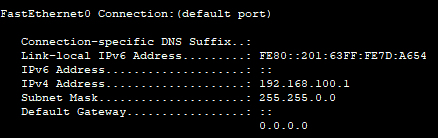
\includegraphics[width=\textwidth,height=\textwidth,keepaspectratio]{./img/aufbau/Server1.png}
        \caption{IP-Config von Server 1}
    \end{subfigure}
    \begin{subfigure}{.7\textwidth}
        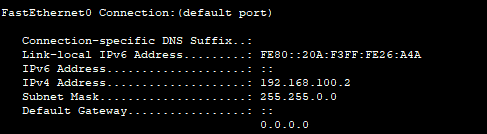
\includegraphics[width=\textwidth,height=.5\textwidth,keepaspectratio]{./img/aufbau/Server2.png}
        \caption{IP-Config von Server 2}
    \end{subfigure}
    \begin{subfigure}{.5\textwidth}
        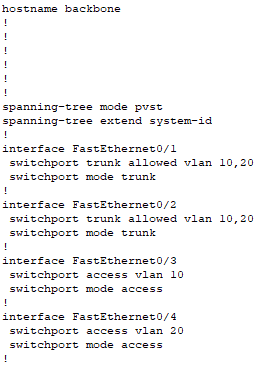
\includegraphics[width=\textwidth,height=1.15\textwidth,keepaspectratio]{./img/aufbau/BB.png}
        \caption{Running Config des Backbone}
    \end{subfigure}
\end{figure}
